\subsubsection{Descripción}

El algoritmo a cada paso tiene un camino $P = [v_1 = u, \dots, v_{i-1}]$ e intenta agregar al camino un nuevo nodo $v_i$ de la adyacencia de $v_{i-1}$, hasta que llega al nodo destino $V$. De esta forma recorre todos los caminos entre $U$ y $V$. De entre todos los caminos tales que el peso por $\omega_1$ es menor o igual a K, se guarda el de menor $\omega_2$.

Se implementaron las siguientes podas:

\begin{itemize}
    \item Se exploran solamente caminos simples. Si un camino tiene ciclos, removiéndolo se obtiene uno con menor longitud tanto en $\omega_1$ como en $\omega_2$. Por lo tanto la solución que buscamos no puede tener ciclos, y nos restringimos a caminos simples. La poda se implementó guardando un arreglo que marca para cada nodo si es parte del camino o no. No se agrega nuevamente si ya es parte del camino.
    \item Si el camino parcial $P = [v_1 = u, \dots, v_{i-1}]$ cumple:

        $omega_1(P)$, sumado a la distancia según $\omega_1$ entre $v_{i-1}$ y $V$, es mayor que $K$

entonces se abandona la rama, es decir, no se recorren los caminos que empiezan en $P$, ya que cualquiera de éstos no va a cumplir con la restricción de que $omega_1$ sea menor o igual a $K$.
    \item Si el camino parcial $P = [v_1 = u, \dots, v_{i-1}]$ cumple:

        $omega_2(P)$, sumado a la distancia según $\omega_2$ entre $v_{i-1}$ y $V$, es mayor o igual que el peso según $\omega_2$ del mejor camino encontrado hasta el momento

entonces se abandona la rama, es decir, no se recorren los caminos que empiezan en $P$, ya que cualquiera de éstos no va a proporcionar una solución mejor que la ya encontrada.
\end{itemize}

Para saber las distancias entre todos los vértices y $v$, al principio se corre dos veces Dijkstra, utilizando como peso primero $\omega_1$ y luego $\omega_2$.

A continuaci\'on, el pseudoc\'odigo de la funci\'on \texttt{backtrack}.

\begin{algorithm}[H]
    \caption{\texttt{backtrack}(Edge e)}
\begin{algorithmic}[1]
  \State Node n $\leftarrow$ e.toNode
  \State currentBranch.path.push\_back(n)
  \State currentBranch.totalOmega1 += e.omega1
  \State currentBranch.totalOmega2 += e.omega2
  \State visited[n] $\leftarrow$ true
  \State podar $\leftarrow$ currentBranch.totalOmega1 + distanceToVOmega1[n] $>$ K \textbf{or} currentBranch.totalOmega2 + distanceToVOmega2[n] $\geq$ bestSolutionFound.totalOmega2
  \If{\textbf{not} podar}
  \If{n = V}
      \State bestSolutionFound $\leftarrow$ currentBranch
  \Else{}
      \For{\textbf{each} Node a \textbf{in} adjacencyList[n] }
	\If{\textbf{not} visited[a] }
          \State Edge f = incidencyMatrix[n][a]
          \State backtrack(f)
	\EndIf
      \EndFor
  \EndIf
  \EndIf
  \State currentBranch.path.pop\_back()
  \State currentBranch.totalOmega1 -= e.omega1
  \State currentBranch.totalOmega2 -= e.omega2
  \State visited[n] $\leftarrow$ false
\end{algorithmic}
\end{algorithm}

\subsubsection{Complejidad}

\fixme{hacer, te tiene que dar (n+1)!}
%Analicemos cuantas llamadas se hacen a $backtrack$. Se exploran caminos de a los sumo $n$ nodos. El primer nodo está fijo en $u$. El segundo nodo
%pertenece a la adyacencia del primero, que en peor caso tiene tamaño $n - 1$. El tercero pertenece a la adyacencia del segundo, que no hayan sido
%visitados, cuyo tamaño es a lo sumo $n - 2$. Y asi sucesivamente. En peor caso se llama a $backtrack$ $n!$ veces.
%
%Analicemos el cómputo que se realiza en cada llamada a $backtrack$. Preguntar si un nodo está visitado es acceder a un arreglo en forma constante.
%El costo de una función de peso asociada a un camino se va acumulando a medida que se agregan nodos. El costo se guarda y se puede acceder en
%forma constante. Lo queda por estudiar es la complejidad del ciclo $for$ que recorre la adyacencia del nodo visitado. Guardamos una lista de
%adyacencia por lo que podemos recorrer la adyacencia de cualquier nodo con complejidad lineal en relación a su tamaño. El tamaño de la adyacencia
%es a lo sumo $m$. Para cada nodo adyacente se efectúan operaciones constantes, a excepción de las llamadas a $backtrack$. El costo de estas
%llamadas lo estamos calculando por separado.
%
%En definitiva hacemos $O(n!)$ llamadas a una función que de por si toma $O(m)$ operaciones. La complejidad del algoritmo es $O(m*n!)$.

\newpage
\subsubsection{Experimentación}

Se efectuó una experimentación sobre el tiempo de ejecución del algoritmo. Primero se evaluó sobre instancias \textit{aleatorias}, de distinto tamaño de entrada. Se obtuvieron dos conclusiones importantes.

Primero, la curva que se puede observar representa una función que crece cada vez más rápido, es decir que no es lineal. Al mismo tiempo, no parece crecer tan rápido como la función factorial que expresa la complejidad teórica del algoritmo.

Segundo, hay mucha amplitud de valores para tamaños de entrada similares. Esto puede deberse a la naturaleza aleatoria de la instancia. Los nodos de origen y destino pueden estar muy cerca o muy lejos, puede haber muchos o pocos caminos entre ellos.

\begin{figure}[H]
    \begin{center}
        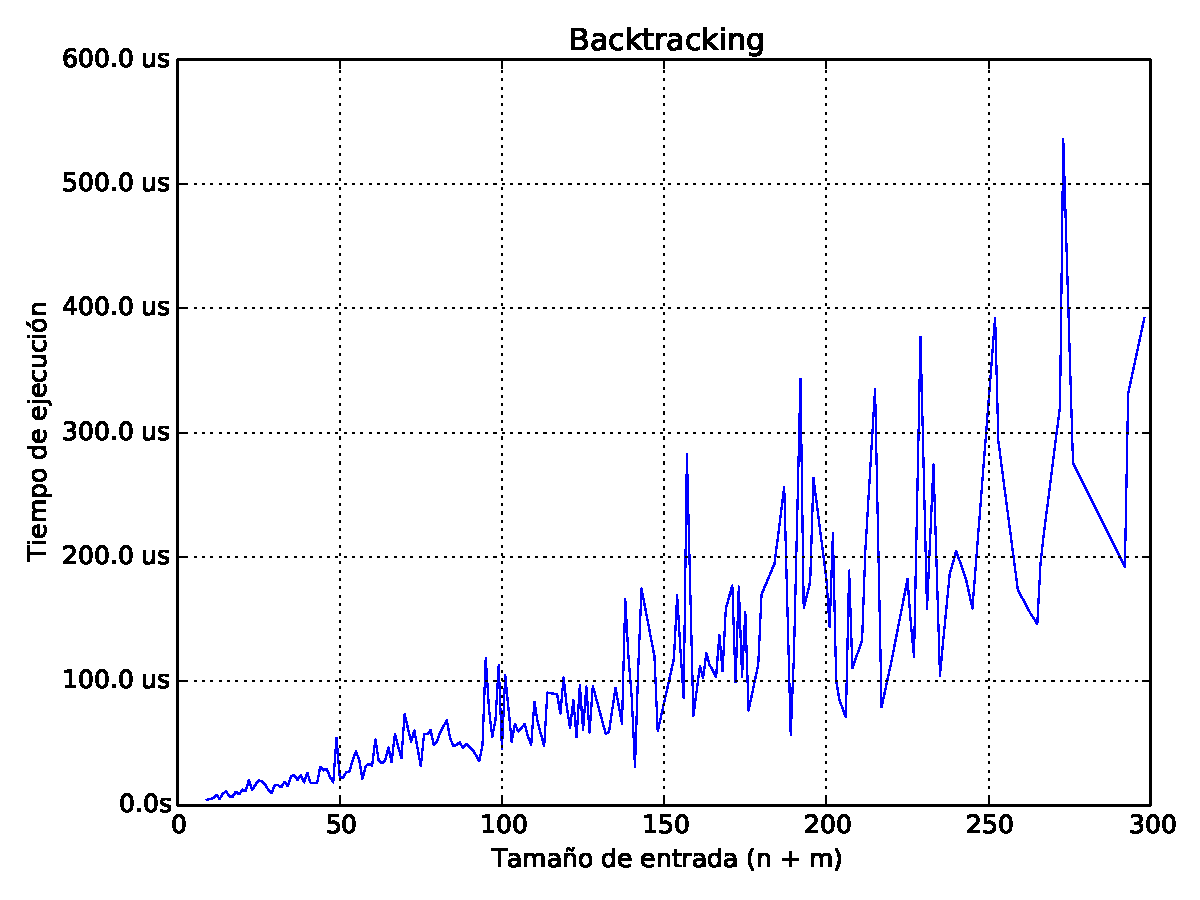
\includegraphics[width=\textwidth]{imagenes/backtracking-complejidad-random.pdf}
        \caption{Tiempo de ejecución de \texttt{backtracking} en instancias \textit{aleatorias}}
    \end{center}
\end{figure}

\newpage
A continuación evaluamos el comportamiento del algoritmo frente a instancias \textit{mágicas}. Se notaron grandes diferencias con la experimentación anterior.

Como primera impresión, se puede observar una curva que parece ser la característica de las funciones factoriales. Los tiempos de ejecución fueron mucho mayores que frente a instancias \textit{aleatorias}. Para los mismos tamaños de entrada, en las últimas no se llegó a tiempos de 1 milisegundo, mientras que en las primeras se superó ampliamente el segundo.

La explicación que se encuentra, según lo desarrollado en la sección de \textit{Generación de instancias}, es que las instancias \textit{mágicas} proveen una gran cantidad de caminos entre $u$ y $v$ que son candidatos a ser el óptimo. Mientras que las instancias \textit{aleatorias} no garantizan ni la lejanía de $u$ y $v$ ni una gran cantidad de caminos candidatos a ser el óptimo. Probablemente una vez que se encuentre el camino las otras ramas de solución se puedan descartar rápidamete.

\begin{figure}[H]
    \begin{center}
        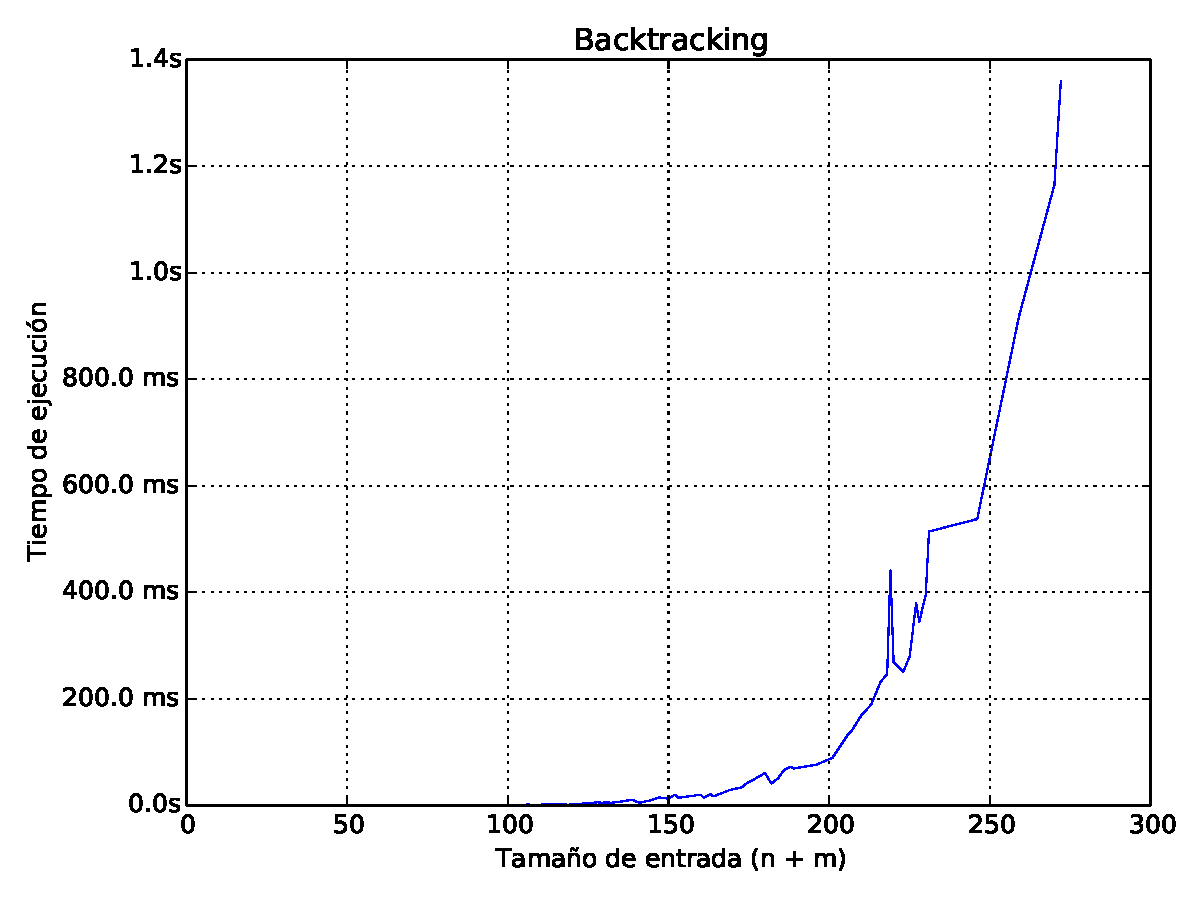
\includegraphics[width=\textwidth]{imagenes/backtracking-complejidad-general.pdf}
        \caption{Tiempo de ejecución de \texttt{backtracking} en instancias \textit{mágicas}}
    \end{center}
\end{figure}

\newpage
Se quiso investigar la performance del algoritmo en relación a $n$, la cantidad de nodos.

Para ello se generaron instancias \textit{mágicas} de distintos valores de $n$, y con $m$ fijo en la mitad de las aristas posibles, es decir $\frac{n(n-1)}{4}$.

Para ver la magnitud de los valores fue apropiada una escala logarítmica. Se puede percibir una muy ligera concavidad positiva de la curva, lo que vendría a indicar que la función crece más rápido que una exponencial(en escala logarítmica toda recta con pendiente $m$ representa la función $m^x$). Con estos resultados se añade evidencia al cálculo de complejidad efectuado, que indica una complejidad factorial en función de $n$.

\begin{figure}[H]
    \begin{center}
        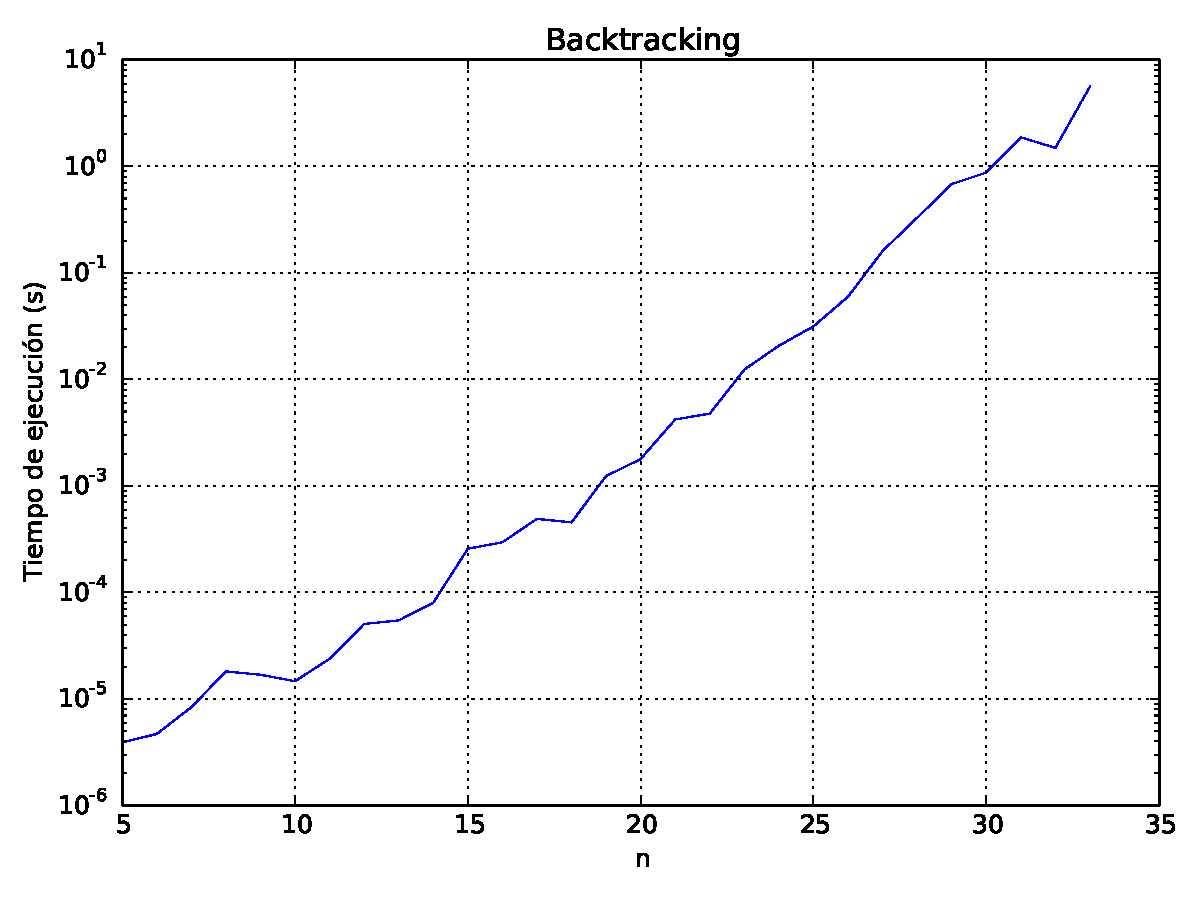
\includegraphics[width=\textwidth]{imagenes/backtracking-complejidad-funcion-de-n.pdf}
        \caption{Tiempo de ejecución de \texttt{backtracking} en instancias \textit{mágicas}, en función de \textit{n}}
    \end{center}
\end{figure}

\newpage
A continuación se exploró el comportamiento del algoritmo en función de $m$, la cantidad de aristas. El valor de $n$ estuvo fijo en 25 y la cantidad de aristas se varió entre $n-1$ y la máxima cantidad para un grafo de 25 vertices.

Nuevamente con escala logarítmica, se observó un gran crecimiento en el tiempo de ejecución a medida que se aumenta $m$. Ésto era predecible ya que se aumenta el tamaño de la adyacencia de los vértices y por lo tanto la cantidad de iteraciones del ciclo en el algoritmo. A más alto nivel, la cantidad de caminos entre $u$ y $v$ tiende a aumentar. Sin embargo, la curva observada tiene concavidad negativa, por lo que representa a una función que crece más lento que una exponencial.

\begin{figure}[H]
    \begin{center}
        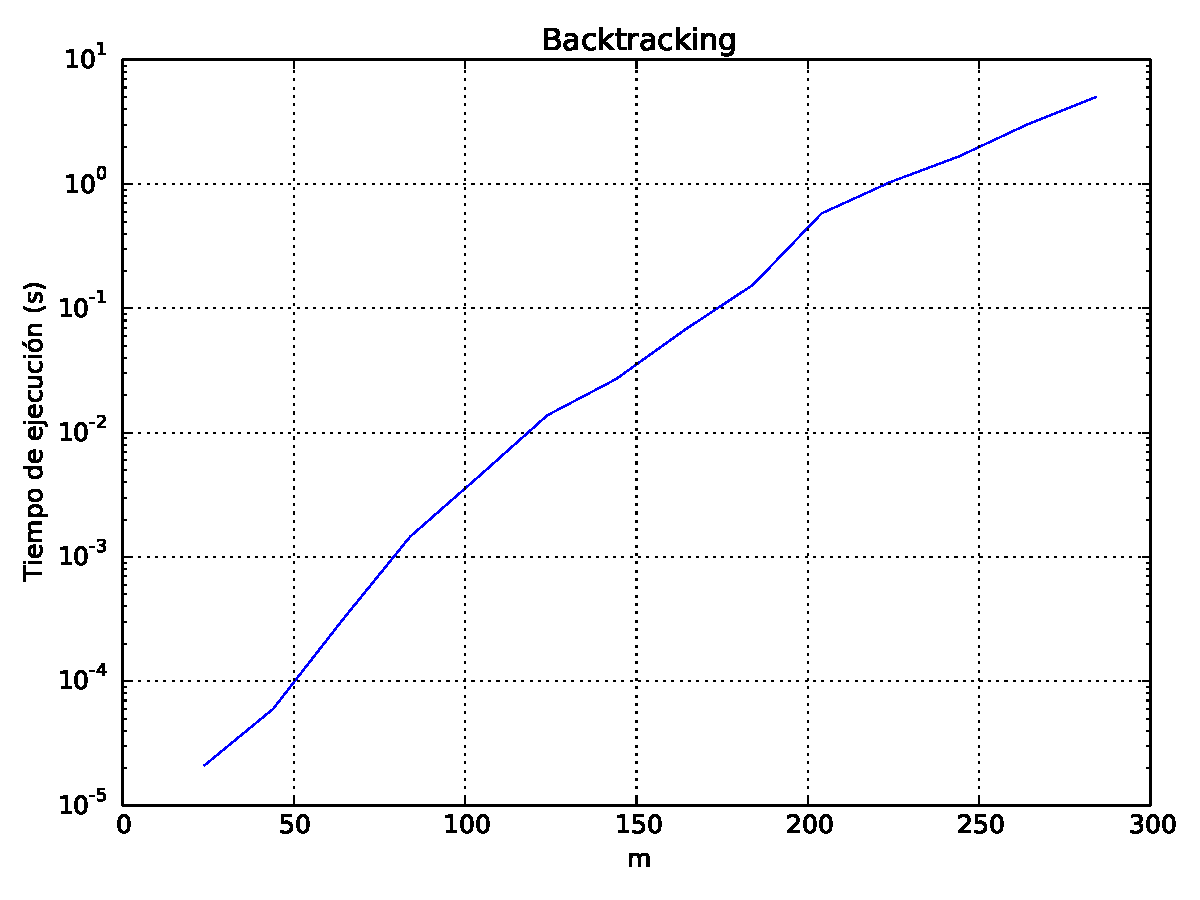
\includegraphics[width=\textwidth]{imagenes/backtracking-complejidad-funcion-de-m.pdf}
        \caption{Tiempo de ejecución de \texttt{backtracking} en instancias \textit{mágicas}, en función de \textit{m}}
    \end{center}
\end{figure}
